%\documentclass{article}
\documentclass[hyperref={colorlinks=true}]{beamer}
%\documentclass[handout,hyperref={colorlinks=true}]{beamer}

\usecolortheme{crane}
\usetheme{Darmstadt}
\usefonttheme{structuresmallcapsserif}
%%%%%%%%%%%%%%%%%%%%%%%%%%%%%%Paquetes%%%%%%%%%%%%%%%%%%%%%%%%%%%%%%%%%%%%%%%%%%%%%%%5
%%%%%%%%%%%%%%%%%%%%%%%%%%%%%%%%%%%%%%%%%%%%%%%%%%%%%%%%%%%%%%%%%%%%%%%%%%%%%%%%%%%%%
%\usepackage{pgfpages}
%\pgfpagesuselayout{2 on 1}[a4paper,border shrink=5mm]
\usepackage{empheq}
\usepackage[spanish]{babel}
\usepackage[utf8x]{inputenc}
\usepackage{times}
%\usepackage[T1]{fontenc}
\usepackage{amssymb,amsmath}
\usepackage{enumerate}
\usepackage{verbatim}
\usepackage{ esint }
%\usepackage{pst-all}
%\usepackage{pstricks-add}
\usepackage{array}
%\usepackage[T1]{fontenc}
\usepackage{animate}
%\usepackage{media9}
\usepackage{xparse}
\usepackage{listings}
\usepackage{ wasysym }
\usepackage{sagetex}
\usepackage{yfonts,mathrsfs,eufrak}
\usepackage{hyperref}

%%%%%%%%%%%%%%%%%%%%%%%%%Configuracion listing
\lstdefinelanguage{Python}
{morekeywords={False,sage,True},sensitive=true}
\lstset{
frame=none,
showtabs=False,
showspaces=False,
showstringspaces=False,
commentstyle={\ttfamily\color{dgreencolor}},
keywordstyle={\ttfamily\color{dbluecolor}\bfseries},
stringstyle={\ttfamily\color{dgraycolor}\bfseries},
language=Python,
basicstyle={\fontsize{8pt}{8pt}\ttfamily},
aboveskip=.3em,
belowskip=0.1em,
numbers=none,
numberstyle=\footnotesize
}

\AtBeginSection[]
{
  \begin{frame}
    \frametitle{Índice}
    \tableofcontents[currentsection]
  \end{frame}
}


%%%%%%%%%%%%%%%%%%%%%%%%Colores
\definecolor{myblue}{rgb}{.8, .8, 1}
\definecolor{dblackcolor}{rgb}{0.0,0.0,0.0}
\definecolor{dbluecolor}{rgb}{0.01,0.02,0.7}
\definecolor{dgreencolor}{rgb}{0.2,0.4,0.0}
\definecolor{dgraycolor}{rgb}{0.30,0.3,0.30}
\newcommand{\dblue}{\color{dbluecolor}\bf}
\newcommand{\dred}{\color{dredcolor}\bf}
\newcommand{\dblack}{\color{dblackcolor}\bf}
%%%%%%%%%%%%%%%%%%%%%%%%%%Nuevos comandos entornos%%%%%%%%%%%%%%%%%%%%%%%%%%%%%%%%
%%%%%%%%%%%%%%%%%%%%%%%%%%%%%%%%%%%%%%%%%%%%%%%%%%%%%%%%%%%%%%%%%%%%%%%%
\newenvironment{demo}{\noindent\emph{Dem.}}{$\square$ \newline\vspace{5pt}}
\newcommand{\com}{\mathbb{C}}
\newcommand{\dis}{\mathbb{D}}
\newcommand{\rr}{\mathbb{R}}
\newcommand{\oo}{\mathcal{O}}
\renewcommand{\emph}[1]{\textcolor[rgb]{1,0,0}{#1}}
\newcommand{\der}[2]{\frac{\partial #1}{\partial #2}}
\renewcommand{\v}[1]{\overrightarrow{#1}}
\renewcommand{\epsilon}{\varepsilon}
\newlength\mytemplen
\newsavebox\mytempbox
\makeatletter
\newcommand\mybluebox{%
\@ifnextchar[%]
{\@mybluebox}%
{\@mybluebox[0pt]}}
\def\@mybluebox[#1]{%
\@ifnextchar[%]
{\@@mybluebox[#1]}%
{\@@mybluebox[#1][0pt]}}
\def\@@mybluebox[#1][#2]#3{
\sbox\mytempbox{#3}%
\mytemplen\ht\mytempbox
\advance\mytemplen #1\relax
\ht\mytempbox\mytemplen
\mytemplen\dp\mytempbox
\advance\mytemplen #2\relax
\dp\mytempbox\mytemplen
\colorbox{myblue}{\hspace{1em}\usebox{\mytempbox}\hspace{1em}}}
\makeatother
\DeclareDocumentCommand\boxedeq{ m g }{%
{\begin{empheq}[box={\mybluebox[2pt][2pt]}]{equation}% #1%
\IfNoValueF {#2} {\label{#2}}%
#1
\end{empheq}
}%
}
\DeclareMathOperator{\atan2}{atan2}
\DeclareMathOperator{\sen}{sen}
\newtheorem{teorema}{Teorema}[section]
\newtheorem{lema}[teorema]{Lema}
\newtheorem{corolario}[teorema]{Corolario}
\newtheorem{proposicion}[teorema]{Proposici\'on}
\newtheorem{definicion}[teorema]{Definici\'on}
%%%%%%%%%%%%%%%%%%%%%%%%%%%%%%%%%%%%%%%%%%%%%%%%%%%%%%%%%%%%%%%%%%%%%%%%%%%%%%%%%%%%%%%%%%%%%%%%%%%%%%%%%%%
%%%%%%%%%%Para escibir en clase articulo o similar
% \usepackage{color}
% \newcommand{\nl}{ }
% \renewenvironment{frame}[1]{}{}
% \newcommand{\qed}{$\square$}
% %\newcommand{\defverbatim}{\def{#1}}
% \newenvironment{block}[1]{\textbf{#1}}{}
% \title{Ecuaciones lineales de segundo orden}
% \author{Fernando Mazzone}
%
%%%%%%%%%%%%%%%%%%%%%%%Para clase beamer
\newcommand{\nl}{\onslide<+-> }

\title[python, SymPy, SAGE] % (optional, nur bei langen Titeln nötig)
{%
\texttt{Python, SymPy} y SAGE
}



\author[] % (optional, nur bei vielen Autoren)
{Fernando Mazzone}

\institute[Depto de Matemática] % (optional, aber oft nötig)
{
 Depto de Matemática\\
Facultad de Ciencias Exactas Físico-Químicas y Naturales\\
Universidad Nacional de Río Cuarto}


\subject{Ecuaciones Diferenciales}

%%%%%%%%%%%%%%%%%%%%%%%%%%%%%%%%%%%%%%%%%%%%%%%%%%%%%%%%%%%%%%%%%%%%%%%%%%%%%%%%%%%%%%


\begin{document}
\begin{frame}
  \maketitle
  \begin{center}
   
\includegraphics[scale=0.2]{imagenes/unrc.jpg}
   \end{center}
\end{frame}
\begin{frame}
    \frametitle{Índice}
\tableofcontents

\end{frame}

\section[Descripción]{Descripción}
\begin{frame}{\texttt{python}}
\begin{tabular}{m{.2\linewidth} m{.8\linewidth} }

\includegraphics[scale=.1]{imagenes/python-logo.png} & \href{https://www.python.org/}{Python} es un lenguaje de programación interpretado, abierto, facil de aprender, potente y portable.\\

\includegraphics[scale=1]{imagenes/scipy_logo.png} & \href{http://www.scipy.org/}{SciPy} Python científico, es un conjunto de módulos para distintos tipos de cálculos. Está integrado por los módulos, SymPy (para cálculos simbólicos), numpy (cálculos numéricos), matplotlib (gráficos) entre otros.  En este curso sólo usaremos SymPy.\\
\end{tabular}
\end{frame}


\begin{frame}{\texttt{python}}
\begin{tabular}{m{.2\linewidth} m{.8\linewidth} }

\includegraphics[scale=.25]{imagenes/sympy_logo.png} & \href{http://www.sympy.org/}{SymPy} 
es una biblioteca de Python para matemática simbólica. Su objetivo es convertirse en un sistema de álgebra computacional (SAC) completo, manteniendo el código lo más simple posible para que sea comprensible y fácilmente extensible. SymPy está escrito enteramente en Python y no requiere de ninguna biblioteca externa.\\


\includegraphics[scale=.13]{imagenes/sage_logo.png} & \href{http://www.sagemath.org/}{SageMath}  es un sistema de software de matemáticas, libre, de código abierto bajo la licencia GPL. Es construído sobre  muchos paquetes de código abierto existentes: NumPy, SciPy, matplotlib, SymPy, Maxima, GAP, FLINT, R y muchos más. Se acceda a su poder combinado a través de un lenguaje común, basado en Python.
\end{tabular}

\end{frame}

\section{Local y online} 

\begin{frame}{Local y online}
\onslide<+->Se pueden usar todos los recursos anteriores de dos formas 
\begin{enumerate}
\item<+-> Instalando el software necesario en una computadora. Nos referiremos a este modo como de acceso local.

\item<+-> A traves de medios online que permiten usar una computadora remota que ejecuta las instrucciones y programas que se tipean en una página web.  Hay varios sitios que ofrecen este servicio. Sugerimos la \href{https://cloud.sagemath.com/}{SageMathCloud}. El usuario debe registrase.
\end{enumerate}
\end{frame}


\section{Instalación} 
\begin{frame}{Instalación local}

Hay mucho software dedicado a gestionar el uso de python, recomendamos las siguientes por la sencillez de la instalación.  

\textbf{Windows} La distribución  \href{https://code.google.com/p/pythonxy/}{python(x,y)}  instala el interprete de python y todos los módulos de scipy. Además el entorno de desarrollo integrado (IDE) spyder. 

Lamentablemente no es posible instalar SageMath en windows, sólo se instala bajo linux.

\textbf{linux} todo es más sencillo, el interprete de python suele venir con la distribución del SO y se puede instalar los módulos, SymPy, NumPy, etc, recurriendo al administrador de paquetes o tipeando la sentencia adecuada en la línea de comandos.  Para instalar SAGE se lo descarga de la página oficial y se descomprime.

\textbf{Otros:} \href{http://ipython.org}{ipython}, \href{http://continuum.io/downloads}{Anaconda}, \href{http://www.gnu.org/software/emacs/}{emacs}.
\end{frame}

\section{scripts, interactivo}
\begin{frame}{Uso}

\onslide<+->Se puede trabajar de dos formas

\begin{enumerate}
\item<+-> Interactivamente, ingresando sentencias a la línea de comandos.

\item<+-> Haciendo un script (programa) donde se guardan todas las sentencias que se desea ejecutar. Posteriormente este script se puede ejecutar desde la línea de comandos o en spyder oprimiendo un botón.

\end{enumerate}



\end{frame}

\section{Características del Lenguaje}
\begin{frame}{Características del Lenguaje}
\onslide<+->Texto extraído de la \href{http://es.wikipedia.org/wiki/Python\#Elementos_del_lenguaje}{wikipedia}
\begin{itemize}
\item<+-> Interpretado
\item<+-> Tipos dinámicos
\item<+->  Multiparadigma, ya que soporta orientación a objetos, programación imperativa y, en menor medida, programación funcional.
\item<+-> Multiplataforma.

\item<+-> Es leído con facilidad. Usa  palabras donde otros lenguajes utilizarían símbolos. Por ejemplo, los operadores lógicos \verb~!, || y \&\&~ en Python se escriben not, or y and, respectivamente.

\end{itemize}

\end{frame}




\begin{frame}{Características del Lenguaje}

\begin{itemize}

\item<+->  El contenido de los bloques de código (bucles, funciones, clases, etc.) es delimitado mediante espacios o tabuladores.

\item<+-> Empieza a contar desde cero (elementos en listas, vectores, etc).



\end{itemize}
\end{frame}



\section{Elementos del Lenguaje}

\defverbatim[colored]\lstI{
\begin{lstlisting}
'''
Comentario  largo en un script de Python
'''
print "Hola mundo" # Comentario corto
\end{lstlisting}
}



\begin{frame}[fragile]{Elementos del Lenguaje}
\textbf{Comentarios}

Dos formas. La primera, para comentarios largos es utilizanda la notación \verb~''' comentario '''~

 La segunda notación utiliza el símbolo \verb~#~, y se extienden hasta el final de la línea.

El intérprete no tiene en cuenta los comentarios, lo cual es útil si deseamos poner información adicional en nuestro código como, por ejemplo, una explicación sobre el comportamiento de una sección del programa.

\lstI


\end{frame}


\defverbatim[colored]\lstI{
\begin{lstlisting}
x = 1
x = "texto" # Esto es posible porque los tipos son asignados \
dinamicamente
\end{lstlisting}
}

\begin{frame}[fragile]{Elementos del Lenguaje}
\textbf{Variables}
Las variables se definen de forma dinámica, lo que significa que no se tiene que especificar cuál es su tipo de antemano y puede tomar distintos valores en otro momento, incluso de un tipo diferente al que tenía previamente. Se usa el símbolo = para asignar valores.

\lstI

El operador \verb+\+ sirve para quebar una línea.

\end{frame}

\defverbatim[colored]\lstI{
\begin{lstlisting}
>>> x=1
>>> type(x)
<type 'int'>
>>> x='Ecuaciones'
>>> type(x)
<type 'str'>
\end{lstlisting}
}

\begin{frame}[fragile]{Elementos del Lenguaje}
\textbf{Tipo de datos}

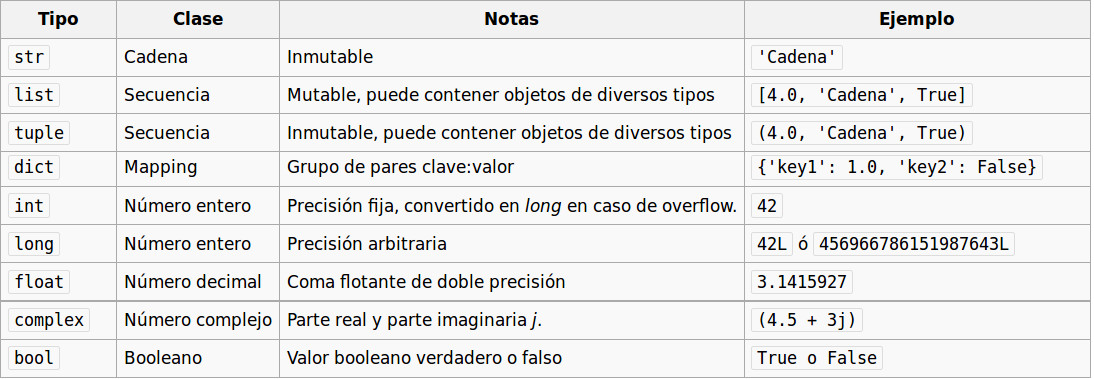
\includegraphics[scale=.4]{imagenes/tipo_datos.jpg}

  \textbf{Mutable:} si su contenido puede cambiarse.

    \textbf{Inmutable:} si su contenido no puede cambiarse.

\lstI

\end{frame}

\begin{frame}{Listas y tuples}

\onslide<+->
\begin{itemize}
\item<+-> Para declarar una lista se usan los corchetes [], en cambio, para declarar una tupla se usan los paréntesis (). En ambas los elementos se separan por comas, y en el caso de las tuplas es necesario que tengan como mínimo una coma.

\item<+->    Tanto las listas como las tuplas pueden contener elementos de diferentes tipos. No obstante las listas suelen usarse para elementos del mismo tipo en cantidad variable mientras que las tuplas se reservan para elementos distintos en cantidad fija.
    
\item<+->Para acceder a los elementos de una lista o tupla se utiliza un índice entero (empezando por "0", no por "1"). Se pueden utilizar índices negativos para acceder elementos a partir del final.


\item<+->Las listas se caracterizan por ser mutables, mientras que las tuplas son inmutables.

\end{itemize}


\end{frame}


\defverbatim[colored]\lstI{
\begin{lstlisting}
>>> lista = ["abc", 42, 3.1415]
>>> lista[0] # Acceder a un elemento por su indice
'abc'
>>> lista[-1] # Acceder a un elemento usando un indice negativo
3.1415
>>> lista.append(True) # Agregar un elemento al final de la lista
>>> lista
['abc', 42, 3.1415, True]
>>> del lista[3] # Borra un elemento de la lista usando un indice 
>>> lista[0] = "xyz" # Re-asignar el valor del primer elemento 
>>> lista[0:2] # elementos del indice "0" al "2" (sin incluir  ultimo)
['xyz', 42]
>>> lista_anidada = [lista, [True, 42L]] # Es posible anidar listas
>>> lista_anidada
[['xyz', 42, 3.1415], [True, 42L]]
>>> lista_anidada[1][0] # Acceder a un elemento de una lista dentro de otra lista
True
\end{lstlisting}
}

\begin{frame}{Listas}
\lstI
\end{frame}

\defverbatim[colored]\lstI{
\begin{lstlisting}
>>> tupla = ("abc", 42, 3.1415)
>>> tupla[0] # Acceder a un elemento por su indice
'abc'
>>> del tupla[0] # No es posible borrar ni agregar
( Excepcion )
>>> tupla[0] = "xyz" # Tampoco es posible re-asignar
( Excepcion )
>>> tupla[0:2] # elementos del indice "0" al "2" sin incluir
('abc', 42)
>>> tupla_anidada = (tupla, (True, 3.1415)) # es posible anidar 
>>> 1, 2, 3, "abc" # Esto tambien es una tupla
(1, 2, 3, 'abc')
>>> (1) #  no es una tupla, ya que no posee al menos una coma
1
>>> (1,) # si es una tupla
(1,)
>>> (1, 2) # Con mas de un elemento no es necesaria la coma final
(1, 2)
>>> (1, 2,) # Aunque agregarla no modifica el resultado
(1, 2)
\end{lstlisting}
}

\begin{frame}{Tuples}
\lstI
\end{frame}

\begin{frame}{Diccionarios}
\begin{itemize}
\item<+->    Para declarar un diccionario se usan las llaves \verb~\{\}~. Contienen elementos separados por comas, donde cada elemento está formado por un par clave:valor (el símbolo : separa la clave de su valor correspondiente).
 \item<+->   Los diccionarios son mutables, es decir, se puede cambiar el contenido de un valor en tiempo de ejecución.
\item<+->    En cambio, las claves de un diccionario deben ser inmutables. Esto quiere decir, por ejemplo, que no podremos usar ni listas ni diccionarios como claves.
\item<+->    El valor asociado a una clave puede ser de cualquier tipo de dato, incluso un diccionario.

\end{itemize}
\end{frame}


\defverbatim[colored]\lstI{
\begin{lstlisting}
>>> dicci = {"cadena": "abc", "numero": 42, "lista": [True, 42L]} 
>>> dicci["cadena"] # Usando una clave, se accede a su valor
'abc'
>>> dicci["lista"][0] 
True
>>> dicci["cadena"] = "xyz" # Re-asignar el valor de una clave
>>> dicci["cadena"]
'xyz'
>>> dicci["decimal"] = 3.1415927 # nuevo elemento clave:valor
>>> dicci["decimal"]
3.1415927
>>> dicci_mixto = {"tupla": (True, 3.1415), "diccionario": dicci}
>>> dicci_mixto["diccionario"]["lista"][1] 
42L
>>> dicci = {("abc",): 42} # tupla puede ser clave pues es inmutable
>>> dicci = {["abc"]: 42} # No es posible que una clave sea una lista
( Excepcion )
\end{lstlisting}
}

\begin{frame}{Diccionarios}
\lstI
\end{frame}






\defverbatim[colored]\lstI{
\begin{lstlisting}
>>> range(5) #  "range" devuelve una lista, empezando en 0 \
y terminando con el numero indicado menos uno
[0, 1, 2, 3, 4]
>>> [i*i for i in range(5)] 
[0, 1, 4, 9, 16]
>>> lista = [(i, i + 2) for i in range(5)]
>>> lista
[(0, 2), (1, 3), (2, 4), (3, 5), (4, 6)]
\end{lstlisting}
}

\begin{frame}{Listas por comprensión}
Una lista por comprensión es una expresión compacta para definir listas. Al igual que el operador lambda, aparece en lenguajes funcionales. Ejemplos:

\lstI
\end{frame}

\defverbatim[colored]\lstI{
\begin{lstlisting}
>>> def suma(x, y = 2):
...     return x + y # Retornar la suma
...
>>> suma(4) # La variable "y" no se modifica, siendo su valor: 2
6
>>> suma(4, 10) # La variable "y" si se modifica
14
\end{lstlisting}
}


\defverbatim[colored]\lstII{
\begin{lstlisting}
>>> suma = lambda x, y = 2: x + y
>>> suma(4) # La variable "y" no se modifica
6
>>> suma(4, 10) # La variable "y" si se modifica
14
\end{lstlisting}
}


\begin{frame}{Funciones}
\begin{itemize}

  \item<+->  Las funciones se definen con la palabra clave def, seguida del nombre de la función y sus parámetros. Otra forma de escribir funciones, aunque menos utilizada, es con la palabra clave lambda (que aparece en lenguajes funcionales como Lisp).
  \item<+->  El valor devuelto en las funciones con def será el dado con la instrucción return.
  \end{itemize}

\end{frame}
\begin{frame}{Funciones}

 \textbf{def}
\lstI
\textbf{lambda}
\lstII
\end{frame}


\begin{frame}{Condicionales}
\textbf{if} Una sentencia condicional (\verb~if~) ejecuta su bloque de código interno sólo si se cumple cierta condición. Se define usando la palabra clave if seguida de la condición, y el bloque de código. Condiciones adicionales, si las hay, se introducen usando elif seguida de la condición y su bloque de código. Todas las condiciones se evalúan secuencialmente hasta encontrar la primera que sea verdadera, y su bloque de código asociado es el único que se ejecuta. Opcionalmente, puede haber un bloque final (la palabra clave else seguida de un bloque de código) que se ejecuta sólo cuando todas las condiciones fueron falsas.

\end{frame}


\defverbatim[colored]\lstI{
\begin{lstlisting}
>>> verdadero = True
>>> if verdadero: # No es necesario poner "verdadero == True"
...     print "Verdadero"
... else:
...     print "Falso"
...
Verdadero
>>> lenguaje = "Python"
>>> if lenguaje == "C": 
...     print "Lenguaje de programacion: C"
... elif lenguaje == "Python": # Se pueden agregar "elif" como se quiera
...     print "Lenguaje de programacion: Python"
... else: 
...     print "Lenguaje de programacion: indefinido"
...
Lenguaje de programacion: Python
>>> if verdadero and lenguaje == "Python": 
...     print "Verdadero y Lenguaje de programacion: Python"
...
Verdadero y Lenguaje de programacion: Python
\end{lstlisting}
}

\begin{frame}{Condicionales}
\lstI
\end{frame}


\defverbatim[colored]\lstI{
\begin{lstlisting}
>>> lista = ["a", "b", "c"]
>>> for i in lista: # Iteramos sobre una lista, que es iterable
...     print i
...
a
b
c
>>> cadena = "abcdef"
>>> for i in cadena: # Iteramos sobre una cadena, que es iterable
...     print i, # una coma al final evita un salto de linea
...
a b c d e f
\end{lstlisting}
}

\begin{frame}{Bucle for}
El bucle for es similar a  otros lenguajes. Recorre un objeto iterable, como una lista, una tupla o un generador, y por cada elemento del iterable ejecuta el bloque de código interno. Se define con la palabra clave for seguida de un nombre de variable, seguido de in, seguido del iterable, y finalmente el bloque de código interno. En cada iteración, el elemento siguiente del iterable se asigna al nombre de variable especificado:
\lstI
\end{frame}



\end{document}





